% Options for packages loaded elsewhere
\PassOptionsToPackage{unicode}{hyperref}
\PassOptionsToPackage{hyphens}{url}
%
\documentclass[
]{article}
\usepackage{amsmath,amssymb}
\usepackage{iftex}
\ifPDFTeX
  \usepackage[T1]{fontenc}
  \usepackage[utf8]{inputenc}
  \usepackage{textcomp} % provide euro and other symbols
\else % if luatex or xetex
  \usepackage{unicode-math} % this also loads fontspec
  \defaultfontfeatures{Scale=MatchLowercase}
  \defaultfontfeatures[\rmfamily]{Ligatures=TeX,Scale=1}
\fi
\usepackage{lmodern}
\ifPDFTeX\else
  % xetex/luatex font selection
\fi
% Use upquote if available, for straight quotes in verbatim environments
\IfFileExists{upquote.sty}{\usepackage{upquote}}{}
\IfFileExists{microtype.sty}{% use microtype if available
  \usepackage[]{microtype}
  \UseMicrotypeSet[protrusion]{basicmath} % disable protrusion for tt fonts
}{}
\makeatletter
\@ifundefined{KOMAClassName}{% if non-KOMA class
  \IfFileExists{parskip.sty}{%
    \usepackage{parskip}
  }{% else
    \setlength{\parindent}{0pt}
    \setlength{\parskip}{6pt plus 2pt minus 1pt}}
}{% if KOMA class
  \KOMAoptions{parskip=half}}
\makeatother
\usepackage{xcolor}
\usepackage[margin=1in]{geometry}
\usepackage{color}
\usepackage{fancyvrb}
\newcommand{\VerbBar}{|}
\newcommand{\VERB}{\Verb[commandchars=\\\{\}]}
\DefineVerbatimEnvironment{Highlighting}{Verbatim}{commandchars=\\\{\}}
% Add ',fontsize=\small' for more characters per line
\usepackage{framed}
\definecolor{shadecolor}{RGB}{248,248,248}
\newenvironment{Shaded}{\begin{snugshade}}{\end{snugshade}}
\newcommand{\AlertTok}[1]{\textcolor[rgb]{0.94,0.16,0.16}{#1}}
\newcommand{\AnnotationTok}[1]{\textcolor[rgb]{0.56,0.35,0.01}{\textbf{\textit{#1}}}}
\newcommand{\AttributeTok}[1]{\textcolor[rgb]{0.13,0.29,0.53}{#1}}
\newcommand{\BaseNTok}[1]{\textcolor[rgb]{0.00,0.00,0.81}{#1}}
\newcommand{\BuiltInTok}[1]{#1}
\newcommand{\CharTok}[1]{\textcolor[rgb]{0.31,0.60,0.02}{#1}}
\newcommand{\CommentTok}[1]{\textcolor[rgb]{0.56,0.35,0.01}{\textit{#1}}}
\newcommand{\CommentVarTok}[1]{\textcolor[rgb]{0.56,0.35,0.01}{\textbf{\textit{#1}}}}
\newcommand{\ConstantTok}[1]{\textcolor[rgb]{0.56,0.35,0.01}{#1}}
\newcommand{\ControlFlowTok}[1]{\textcolor[rgb]{0.13,0.29,0.53}{\textbf{#1}}}
\newcommand{\DataTypeTok}[1]{\textcolor[rgb]{0.13,0.29,0.53}{#1}}
\newcommand{\DecValTok}[1]{\textcolor[rgb]{0.00,0.00,0.81}{#1}}
\newcommand{\DocumentationTok}[1]{\textcolor[rgb]{0.56,0.35,0.01}{\textbf{\textit{#1}}}}
\newcommand{\ErrorTok}[1]{\textcolor[rgb]{0.64,0.00,0.00}{\textbf{#1}}}
\newcommand{\ExtensionTok}[1]{#1}
\newcommand{\FloatTok}[1]{\textcolor[rgb]{0.00,0.00,0.81}{#1}}
\newcommand{\FunctionTok}[1]{\textcolor[rgb]{0.13,0.29,0.53}{\textbf{#1}}}
\newcommand{\ImportTok}[1]{#1}
\newcommand{\InformationTok}[1]{\textcolor[rgb]{0.56,0.35,0.01}{\textbf{\textit{#1}}}}
\newcommand{\KeywordTok}[1]{\textcolor[rgb]{0.13,0.29,0.53}{\textbf{#1}}}
\newcommand{\NormalTok}[1]{#1}
\newcommand{\OperatorTok}[1]{\textcolor[rgb]{0.81,0.36,0.00}{\textbf{#1}}}
\newcommand{\OtherTok}[1]{\textcolor[rgb]{0.56,0.35,0.01}{#1}}
\newcommand{\PreprocessorTok}[1]{\textcolor[rgb]{0.56,0.35,0.01}{\textit{#1}}}
\newcommand{\RegionMarkerTok}[1]{#1}
\newcommand{\SpecialCharTok}[1]{\textcolor[rgb]{0.81,0.36,0.00}{\textbf{#1}}}
\newcommand{\SpecialStringTok}[1]{\textcolor[rgb]{0.31,0.60,0.02}{#1}}
\newcommand{\StringTok}[1]{\textcolor[rgb]{0.31,0.60,0.02}{#1}}
\newcommand{\VariableTok}[1]{\textcolor[rgb]{0.00,0.00,0.00}{#1}}
\newcommand{\VerbatimStringTok}[1]{\textcolor[rgb]{0.31,0.60,0.02}{#1}}
\newcommand{\WarningTok}[1]{\textcolor[rgb]{0.56,0.35,0.01}{\textbf{\textit{#1}}}}
\usepackage{graphicx}
\makeatletter
\def\maxwidth{\ifdim\Gin@nat@width>\linewidth\linewidth\else\Gin@nat@width\fi}
\def\maxheight{\ifdim\Gin@nat@height>\textheight\textheight\else\Gin@nat@height\fi}
\makeatother
% Scale images if necessary, so that they will not overflow the page
% margins by default, and it is still possible to overwrite the defaults
% using explicit options in \includegraphics[width, height, ...]{}
\setkeys{Gin}{width=\maxwidth,height=\maxheight,keepaspectratio}
% Set default figure placement to htbp
\makeatletter
\def\fps@figure{htbp}
\makeatother
\setlength{\emergencystretch}{3em} % prevent overfull lines
\providecommand{\tightlist}{%
  \setlength{\itemsep}{0pt}\setlength{\parskip}{0pt}}
\setcounter{secnumdepth}{-\maxdimen} % remove section numbering
\usepackage{float} \floatplacement{figure}{H}
\ifLuaTeX
  \usepackage{selnolig}  % disable illegal ligatures
\fi
\IfFileExists{bookmark.sty}{\usepackage{bookmark}}{\usepackage{hyperref}}
\IfFileExists{xurl.sty}{\usepackage{xurl}}{} % add URL line breaks if available
\urlstyle{same}
\hypersetup{
  pdftitle={Report for SURV675 Assignment 3},
  pdfauthor={Becky Yuen},
  hidelinks,
  pdfcreator={LaTeX via pandoc}}

\title{Report for SURV675 Assignment 3}
\author{Becky Yuen}
\date{}

\begin{document}
\maketitle

\hypertarget{introduction}{%
\subsection{Introduction}\label{introduction}}

This is the overall report for the analysis on the trend of COVID-19
cases over the past few years. All data are downloaded from
\href{https://github.com/CSSEGISandData/COVID-19/tree/master/csse_covid_19_data}{JHU
CSSE COVID-19 Dataset}.

\begin{Shaded}
\begin{Highlighting}[]
\FunctionTok{library}\NormalTok{(sparklyr)}
\FunctionTok{library}\NormalTok{(dplyr)}
\NormalTok{sc }\OtherTok{\textless{}{-}} \FunctionTok{spark\_connect}\NormalTok{(}\AttributeTok{master =} \StringTok{"local"}\NormalTok{)}
\end{Highlighting}
\end{Shaded}

\hypertarget{prepare-data-set-in-spark}{%
\subsection{Prepare data set in Spark}\label{prepare-data-set-in-spark}}

\begin{enumerate}
\def\labelenumi{\arabic{enumi}.}
\tightlist
\item
  Download data
\end{enumerate}

\begin{Shaded}
\begin{Highlighting}[]
\FunctionTok{library}\NormalTok{(readr)}

\NormalTok{data\_path }\OtherTok{=} 
  \StringTok{"https://raw.githubusercontent.com/CSSEGISandData/COVID{-}19/master/csse\_covid\_19\_data/"}

\NormalTok{urlfile }\OtherTok{=} \FunctionTok{paste}\NormalTok{(data\_path,}\StringTok{"UID\_ISO\_FIPS\_LookUp\_Table.csv"}\NormalTok{,}\AttributeTok{collapse=}\StringTok{""}\NormalTok{)}
\NormalTok{urlfile1 }\OtherTok{=} \FunctionTok{paste}\NormalTok{(data\_path,}
      \StringTok{"csse\_covid\_19\_time\_series/time\_series\_covid19\_confirmed\_global.csv"}\NormalTok{,}\AttributeTok{collapse=}\StringTok{""}\NormalTok{)}

\NormalTok{LookUp\_Table\_R }\OtherTok{=} \FunctionTok{read\_csv}\NormalTok{(}\FunctionTok{url}\NormalTok{(urlfile))}
\NormalTok{time\_series\_R }\OtherTok{=} \FunctionTok{read\_csv}\NormalTok{(}\FunctionTok{url}\NormalTok{(urlfile1))}

\FunctionTok{names}\NormalTok{(LookUp\_Table\_R)[}\FunctionTok{which}\NormalTok{(}\FunctionTok{names}\NormalTok{(LookUp\_Table\_R)}\SpecialCharTok{==}\StringTok{"Long\_"}\NormalTok{)] }\OtherTok{=} \StringTok{"Long"}
\FunctionTok{names}\NormalTok{(time\_series\_R)[}\FunctionTok{which}\NormalTok{(}\FunctionTok{names}\NormalTok{(time\_series\_R)}\SpecialCharTok{==}\StringTok{"Province/State"}\NormalTok{)] }\OtherTok{=} \StringTok{"Province\_State"}
\FunctionTok{names}\NormalTok{(time\_series\_R)[}\FunctionTok{which}\NormalTok{(}\FunctionTok{names}\NormalTok{(time\_series\_R)}\SpecialCharTok{==}\StringTok{"Country/Region"}\NormalTok{)] }\OtherTok{=} \StringTok{"Country\_Region"}

\FunctionTok{names}\NormalTok{(time\_series\_R)[}\DecValTok{5}\SpecialCharTok{:}\FunctionTok{dim}\NormalTok{(time\_series\_R)[}\DecValTok{2}\NormalTok{]] }\OtherTok{=} 
  \FunctionTok{as.character}\NormalTok{(}\FunctionTok{as.numeric}\NormalTok{(lubridate}\SpecialCharTok{::}\FunctionTok{mdy}\NormalTok{(}\FunctionTok{names}\NormalTok{(time\_series\_R)[}\DecValTok{5}\SpecialCharTok{:}\FunctionTok{dim}\NormalTok{(time\_series\_R)[}\DecValTok{2}\NormalTok{]])))}
\end{Highlighting}
\end{Shaded}

\begin{enumerate}
\def\labelenumi{\arabic{enumi}.}
\setcounter{enumi}{1}
\tightlist
\item
  Upload data to spark
\end{enumerate}

\begin{Shaded}
\begin{Highlighting}[]
\NormalTok{LookUp\_Table }\OtherTok{=} \FunctionTok{copy\_to}\NormalTok{(sc, UID\_ISO\_FIPS\_LookUp\_Table, }\AttributeTok{overwrite =} \ConstantTok{TRUE}\NormalTok{)}
\NormalTok{time\_series }\OtherTok{=} \FunctionTok{copy\_to}\NormalTok{(sc, time\_series\_covid19\_confirmed\_global, }\AttributeTok{overwrite =} \ConstantTok{TRUE}\NormalTok{)}
\end{Highlighting}
\end{Shaded}

\begin{enumerate}
\def\labelenumi{\arabic{enumi}.}
\setcounter{enumi}{2}
\tightlist
\item
  Merge data sets and select countries in Spark
\end{enumerate}

\begin{Shaded}
\begin{Highlighting}[]
\NormalTok{All\_data }\OtherTok{=} \FunctionTok{inner\_join}\NormalTok{(time\_series, LookUp\_Table, }\AttributeTok{by =} \FunctionTok{c}\NormalTok{(}\StringTok{"Country\_Region"}\NormalTok{,}\StringTok{"Lat"}\NormalTok{,}\StringTok{"Long"}\NormalTok{))}

\NormalTok{All\_data\_country }\OtherTok{=} \FunctionTok{sdf\_copy\_to}\NormalTok{(sc, All\_data) }\SpecialCharTok{\%\textgreater{}\%} \FunctionTok{filter}\NormalTok{(Country\_Region}\SpecialCharTok{\%in\%}
                  \FunctionTok{c}\NormalTok{(}\StringTok{"Germany"}\NormalTok{,}\StringTok{"China"}\NormalTok{,}\StringTok{"Japan"}\NormalTok{,}\StringTok{"United Kingdom"}\NormalTok{,}\StringTok{"US"}\NormalTok{,}\StringTok{"Brail"}\NormalTok{,}\StringTok{"Mexico"}\NormalTok{))}
\end{Highlighting}
\end{Shaded}

\begin{enumerate}
\def\labelenumi{\arabic{enumi}.}
\setcounter{enumi}{3}
\tightlist
\item
  Transform data set from wide to long
\end{enumerate}

\begin{Shaded}
\begin{Highlighting}[]
\NormalTok{All\_data\_long\_country }\OtherTok{=} \FunctionTok{reshape}\NormalTok{(}\AttributeTok{data =}\NormalTok{ tibble}\SpecialCharTok{::}\FunctionTok{as\_tibble}\NormalTok{(All\_data\_country),}
                                \AttributeTok{idvar=} \StringTok{"UID"}\NormalTok{,}
                                \AttributeTok{varying =} \FunctionTok{colnames}\NormalTok{(All\_data\_country)[}\DecValTok{5}\SpecialCharTok{:}\DecValTok{1147}\NormalTok{], }
                                \AttributeTok{v.names =} \StringTok{"n\_case"}\NormalTok{,}
                                \AttributeTok{timevar=} \StringTok{"date"}\NormalTok{,}
                                \AttributeTok{times =} \FunctionTok{colnames}\NormalTok{(All\_data\_country)[}\DecValTok{5}\SpecialCharTok{:}\DecValTok{1147}\NormalTok{], }
                                \AttributeTok{new.row.names =} \DecValTok{1}\SpecialCharTok{:}\DecValTok{320040}\NormalTok{,}
                                \AttributeTok{direction =} \StringTok{"long"}\NormalTok{)}
\end{Highlighting}
\end{Shaded}

\hypertarget{graphs}{%
\subsection{Graphs}\label{graphs}}

\begin{Shaded}
\begin{Highlighting}[]
\FunctionTok{library}\NormalTok{(ggplot2)}
\FunctionTok{library}\NormalTok{(tidyr)}
\FunctionTok{library}\NormalTok{(dplyr)}
\FunctionTok{library}\NormalTok{(lubridate, }\AttributeTok{warn.conflicts =} \ConstantTok{FALSE}\NormalTok{)}

\FunctionTok{names}\NormalTok{(All\_data\_long\_country)[}\FunctionTok{which}\NormalTok{(}\FunctionTok{names}\NormalTok{(All\_data\_long\_country)}\SpecialCharTok{==}\StringTok{"date"}\NormalTok{)] }\OtherTok{=} \StringTok{"date\_int"}
\NormalTok{All\_data\_long\_country}\SpecialCharTok{$}\NormalTok{date }\OtherTok{=} \FunctionTok{as.Date}\NormalTok{(}\FunctionTok{as.numeric}\NormalTok{(All\_data\_long\_country}\SpecialCharTok{$}\NormalTok{date\_int))}

\NormalTok{All\_data\_long\_date\_country }\OtherTok{=}\NormalTok{ All\_data\_long\_country }\SpecialCharTok{\%\textgreater{}\%} 
                              \FunctionTok{group\_by}\NormalTok{(date, Country\_Region) }\SpecialCharTok{\%\textgreater{}\%} 
                              \FunctionTok{summarize}\NormalTok{(}\AttributeTok{ncase\_bydate =} \FunctionTok{sum}\NormalTok{(n\_case), }
                                        \AttributeTok{total\_population =} \FunctionTok{sum}\NormalTok{(Population)) }\SpecialCharTok{\%\textgreater{}\%} 
                              \FunctionTok{arrange}\NormalTok{(date) }
\end{Highlighting}
\end{Shaded}

\begin{Shaded}
\begin{Highlighting}[]
\NormalTok{graph2 }\OtherTok{=} \FunctionTok{ggplot}\NormalTok{(}\AttributeTok{data =}\NormalTok{ All\_data\_long\_date\_country, }\AttributeTok{mapping =} \FunctionTok{aes}\NormalTok{(}\AttributeTok{x =}\NormalTok{ date, }\AttributeTok{y =} \FunctionTok{log}\NormalTok{(ncase\_bydate)))}
\NormalTok{(}\AttributeTok{fig2 =}\NormalTok{ graph2 }\SpecialCharTok{+} \FunctionTok{geom\_line}\NormalTok{(}\FunctionTok{aes}\NormalTok{(}\AttributeTok{group =}\NormalTok{ Country\_Region)) }\SpecialCharTok{+} 
    \FunctionTok{labs}\NormalTok{(}\AttributeTok{x =} \StringTok{"Date"}\NormalTok{, }\AttributeTok{y =} \StringTok{"Number of cases (in log form)"}\NormalTok{, }
         \AttributeTok{title =} \StringTok{"Change of number of cases (in log form) by Country"}\NormalTok{))}
\end{Highlighting}
\end{Shaded}

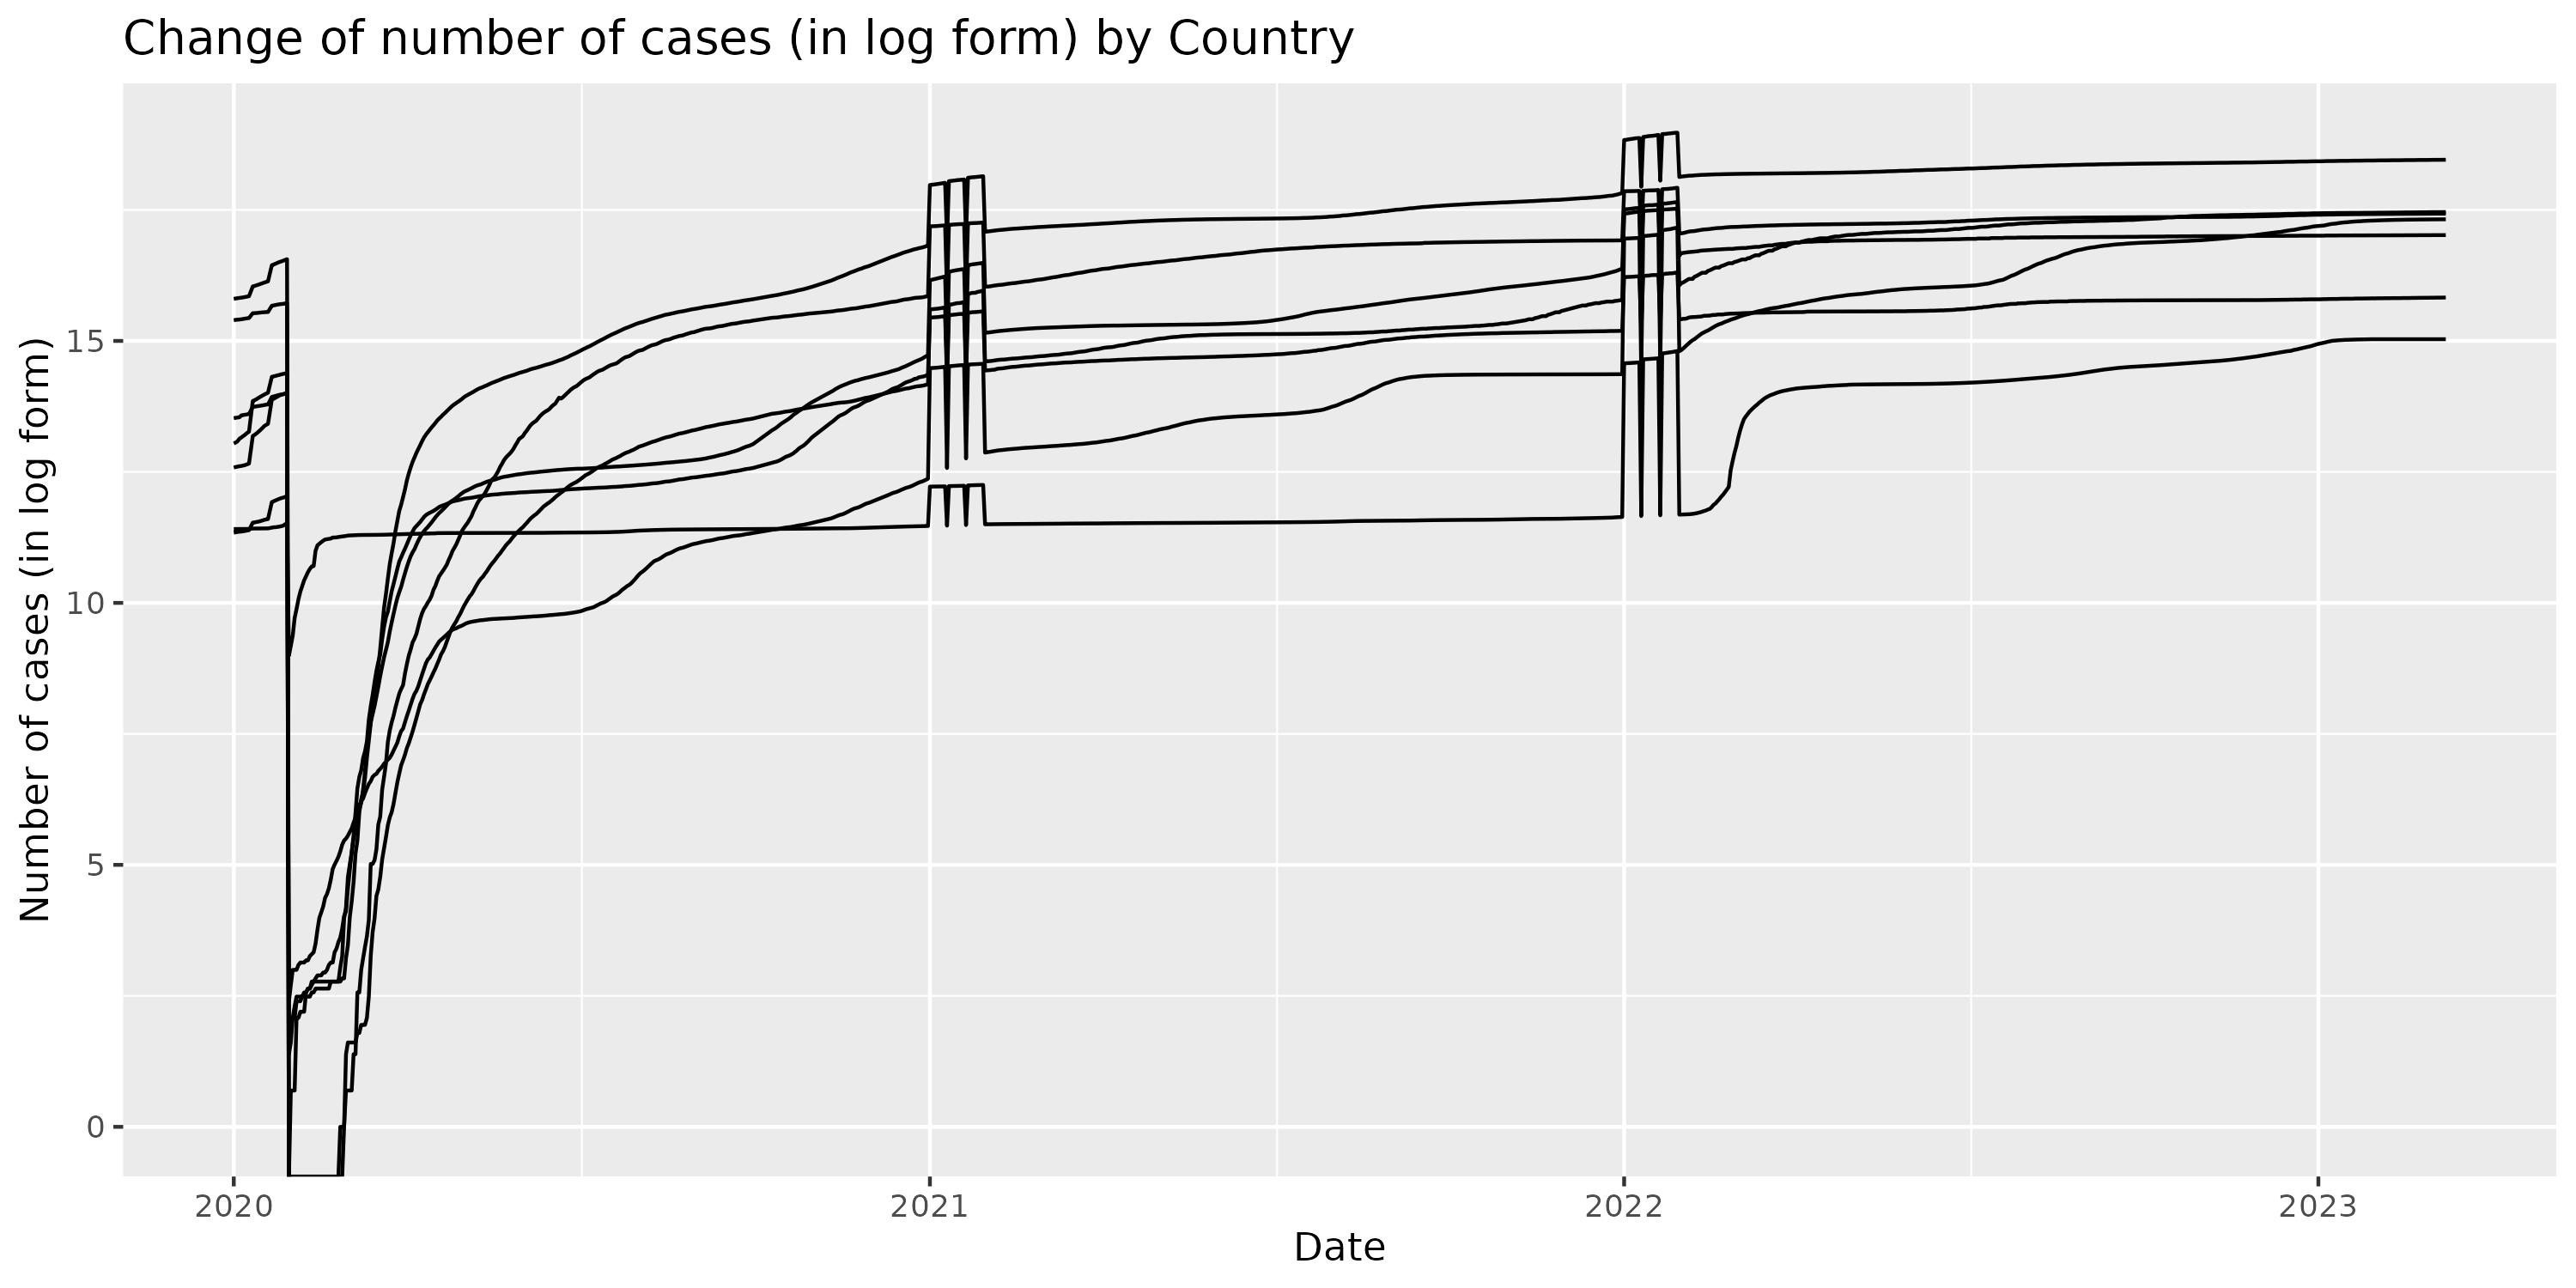
\includegraphics{./fig2.jpeg} We can see that the trends in different
countries are similar.\\

\begin{Shaded}
\begin{Highlighting}[]
\NormalTok{graph3 }\OtherTok{=} \FunctionTok{ggplot}\NormalTok{(}\AttributeTok{data =}\NormalTok{ All\_data\_long\_date\_country, }\AttributeTok{mapping =} \FunctionTok{aes}\NormalTok{(}\AttributeTok{x =}\NormalTok{ date, }\AttributeTok{y =}\NormalTok{ ncase\_bydate}\SpecialCharTok{/}\NormalTok{total\_population))}
\NormalTok{(}\AttributeTok{fig3 =}\NormalTok{ graph3 }\SpecialCharTok{+} \FunctionTok{geom\_line}\NormalTok{(}\FunctionTok{aes}\NormalTok{(}\AttributeTok{group =}\NormalTok{ Country\_Region)) }\SpecialCharTok{+} 
    \FunctionTok{labs}\NormalTok{(}\AttributeTok{x =} \StringTok{"Date"}\NormalTok{, }\AttributeTok{y =} \StringTok{"Incident Rate"}\NormalTok{, }
         \AttributeTok{title =} \StringTok{"Change of Incident Rate (cases per total population) by Country"}\NormalTok{))}
\end{Highlighting}
\end{Shaded}

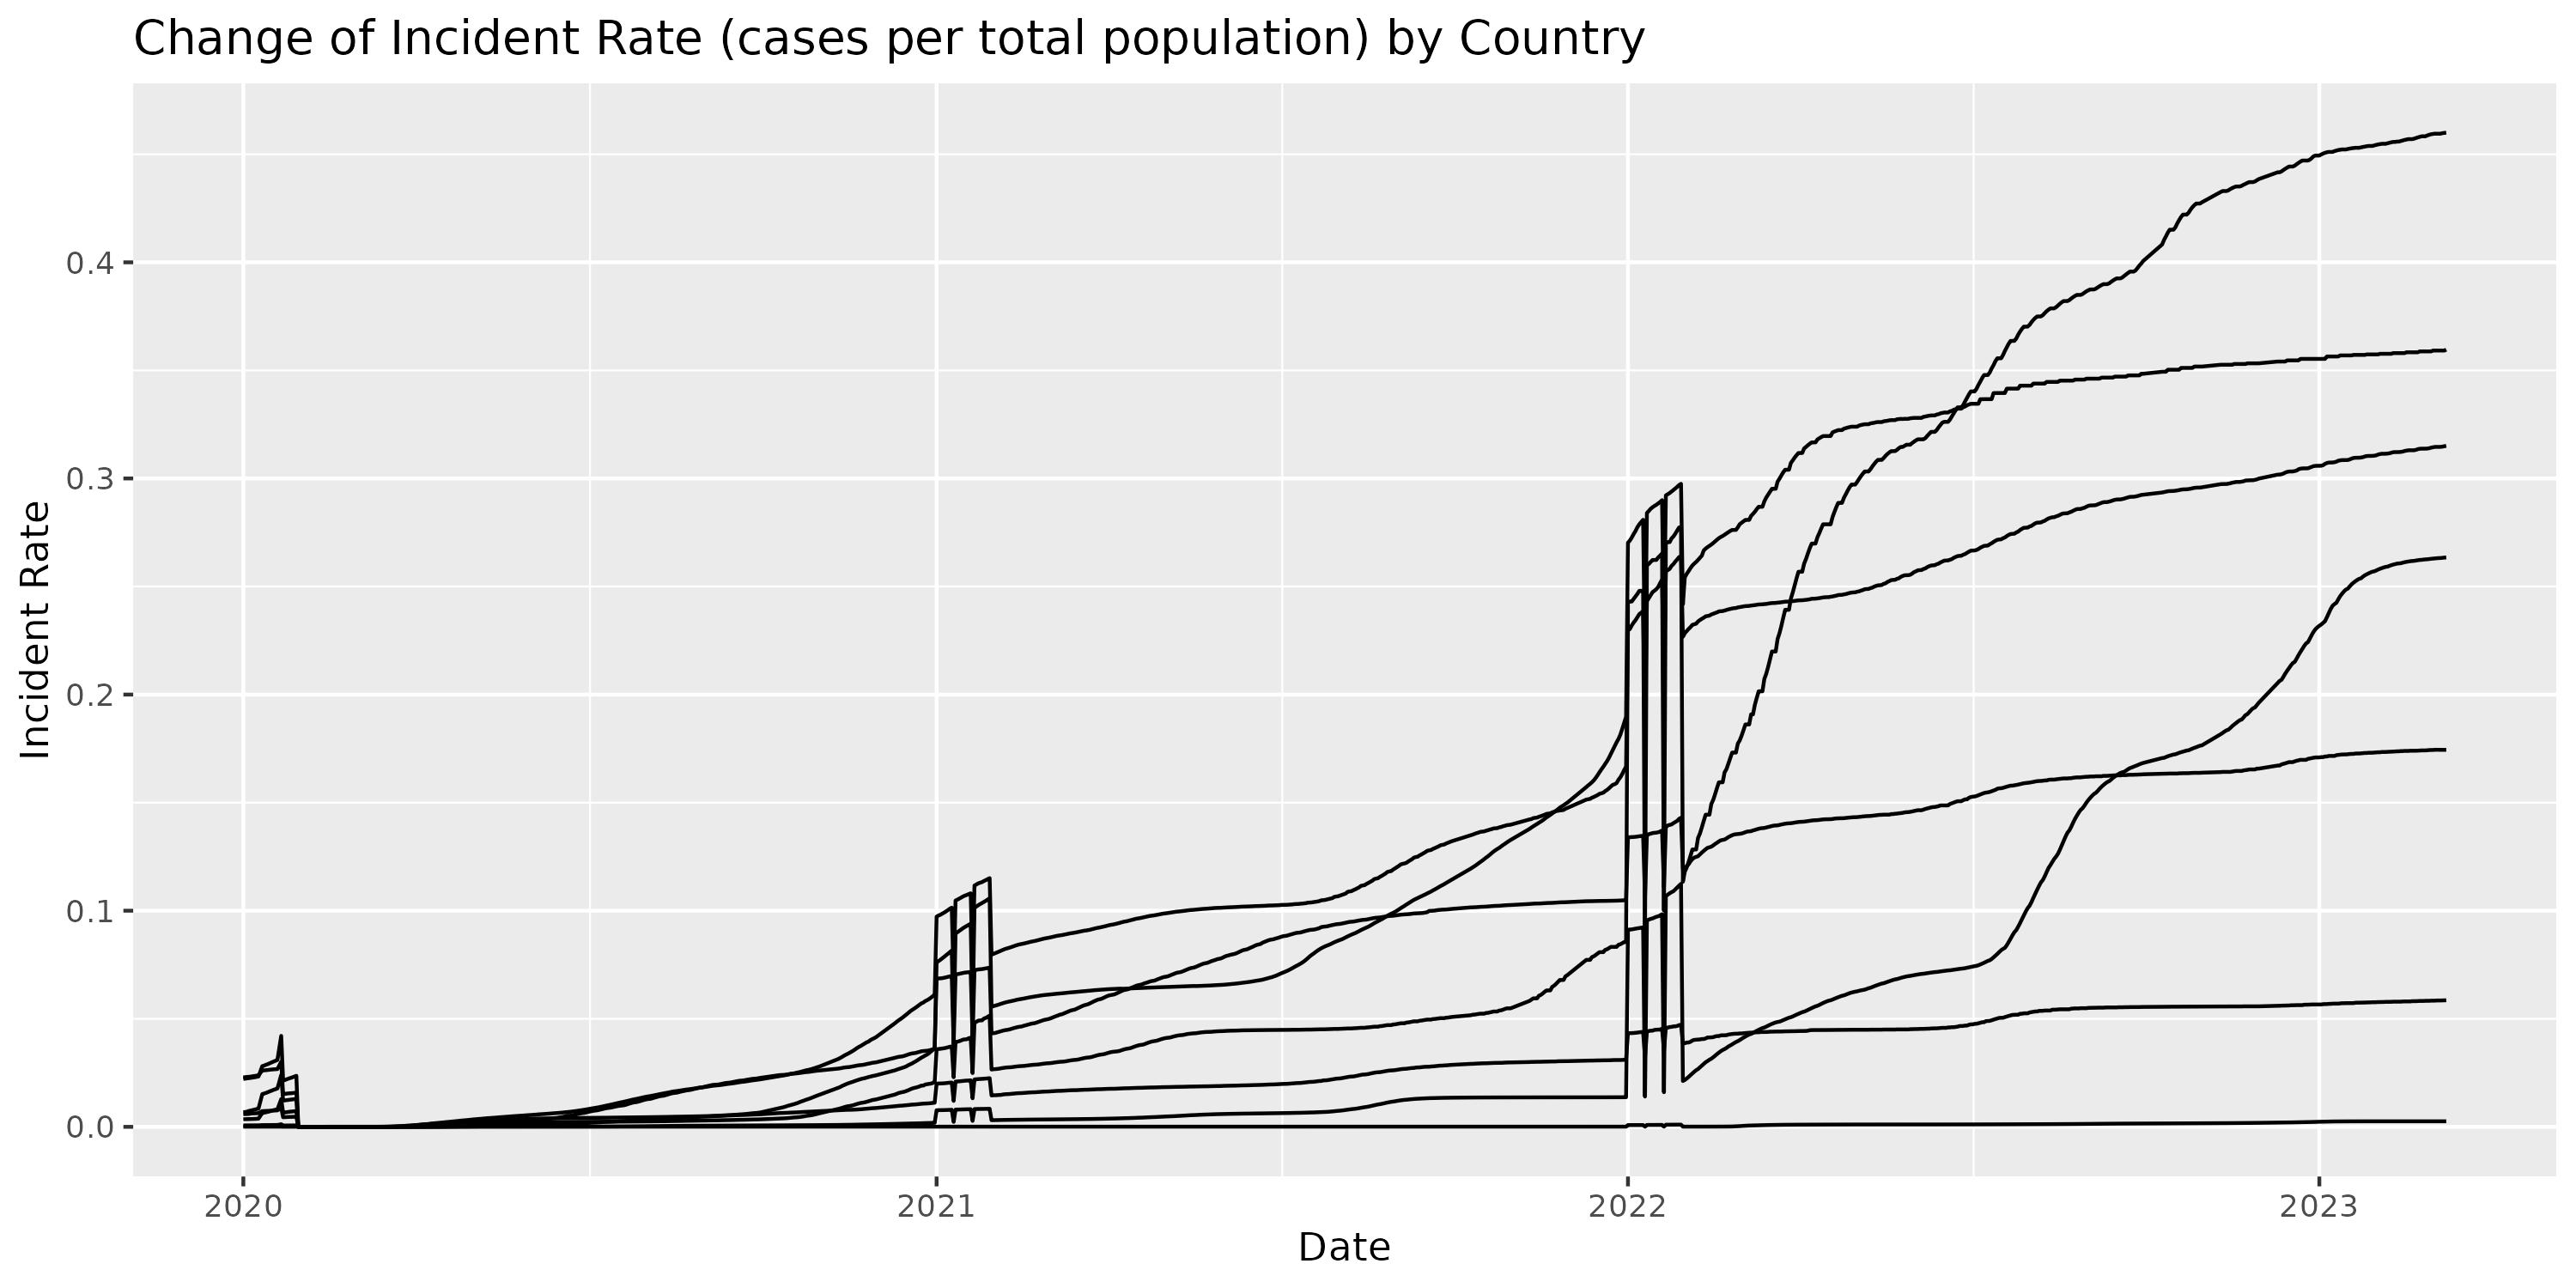
\includegraphics{./fig3.jpeg} That being said, the change in incident
rates differs among different countries.

\hypertarget{regression-analysis-in-spark}{%
\subsection{Regression Analysis in
Spark}\label{regression-analysis-in-spark}}

\hypertarget{model-logleft-textnumber-of-cases-right-population-number-of-days-since-covid-begins-country}{%
\subsubsection{\texorpdfstring{Model:
\(\log\left\{ \text{number of cases} \right\}\) \textasciitilde{}
Population + Number of days since COVID begins +
Country}{Model: \textbackslash log\textbackslash left\textbackslash\{ \textbackslash text\{number of cases\} \textbackslash right\textbackslash\} \textasciitilde{} Population + Number of days since COVID begins + Country}}\label{model-logleft-textnumber-of-cases-right-population-number-of-days-since-covid-begins-country}}

\begin{Shaded}
\begin{Highlighting}[]
\NormalTok{All\_data\_long\_country}\SpecialCharTok{$}\NormalTok{ndays\_since\_covid }\OtherTok{=} 
  \FunctionTok{as.numeric}\NormalTok{(All\_data\_long\_country}\SpecialCharTok{$}\NormalTok{date }\SpecialCharTok{{-}} \FunctionTok{sort}\NormalTok{(All\_data\_long\_country}\SpecialCharTok{$}\NormalTok{date)[}\DecValTok{1}\NormalTok{])}
\NormalTok{All\_data\_long\_country }\OtherTok{=}\NormalTok{ All\_data\_long\_country[}\SpecialCharTok{{-}}\FunctionTok{which}\NormalTok{(All\_data\_long\_country}\SpecialCharTok{$}\NormalTok{n\_case}\SpecialCharTok{==}\DecValTok{0}\NormalTok{),]}
\NormalTok{All\_data\_long\_country}\SpecialCharTok{$}\NormalTok{log\_n\_case }\OtherTok{=} \FunctionTok{log}\NormalTok{(All\_data\_long\_country}\SpecialCharTok{$}\NormalTok{n\_case)}
\NormalTok{All\_data\_long\_country }\OtherTok{=}\NormalTok{ All\_data\_long\_country[}\SpecialCharTok{{-}}\FunctionTok{which}\NormalTok{(All\_data\_long\_country}\SpecialCharTok{$}\NormalTok{log\_n\_case}\SpecialCharTok{==}\DecValTok{0}\NormalTok{),]}

\DocumentationTok{\#\# US as reference}
\NormalTok{All\_data\_long\_country}\SpecialCharTok{$}\NormalTok{China }\OtherTok{=}\NormalTok{ (All\_data\_long\_country}\SpecialCharTok{$}\NormalTok{Country\_Region}\SpecialCharTok{==}\StringTok{"China"}\NormalTok{)}\SpecialCharTok{+}\DecValTok{0}
\NormalTok{All\_data\_long\_country}\SpecialCharTok{$}\NormalTok{Germany }\OtherTok{=}\NormalTok{ (All\_data\_long\_country}\SpecialCharTok{$}\NormalTok{Country\_Region}\SpecialCharTok{==}\StringTok{"Germany"}\NormalTok{)}\SpecialCharTok{+}\DecValTok{0}
\NormalTok{All\_data\_long\_country}\SpecialCharTok{$}\NormalTok{Japan }\OtherTok{=}\NormalTok{ (All\_data\_long\_country}\SpecialCharTok{$}\NormalTok{Country\_Region}\SpecialCharTok{==}\StringTok{"Japan"}\NormalTok{)}\SpecialCharTok{+}\DecValTok{0}
\NormalTok{All\_data\_long\_country}\SpecialCharTok{$}\NormalTok{Mexico }\OtherTok{=}\NormalTok{ (All\_data\_long\_country}\SpecialCharTok{$}\NormalTok{Country\_Region}\SpecialCharTok{==}\StringTok{"Mexico"}\NormalTok{)}\SpecialCharTok{+}\DecValTok{0}
\NormalTok{All\_data\_long\_country}\SpecialCharTok{$}\NormalTok{UK }\OtherTok{=}\NormalTok{ (All\_data\_long\_country}\SpecialCharTok{$}\NormalTok{Country\_Region}\SpecialCharTok{==}\StringTok{"United Kingdom"}\NormalTok{)}\SpecialCharTok{+}\DecValTok{0}

\NormalTok{All\_data\_long\_country }\OtherTok{=}\NormalTok{ All\_data\_long\_country[,}\FunctionTok{which}\NormalTok{(}\FunctionTok{colnames}\NormalTok{(All\_data\_long\_country)}\SpecialCharTok{\%in\%}
                        \FunctionTok{c}\NormalTok{(}\StringTok{"Population"}\NormalTok{,}\StringTok{"log\_n\_case"}\NormalTok{,}\StringTok{"ndays\_since\_covid"}\NormalTok{,}\StringTok{"China"}\NormalTok{,}
                          \StringTok{"Germany"}\NormalTok{,}\StringTok{"Japan"}\NormalTok{,}\StringTok{"Mexico"}\NormalTok{,}\StringTok{"United Kingdom"}\NormalTok{))]}
\NormalTok{All\_data\_long\_country\_lm }\OtherTok{=}
\NormalTok{  All\_data\_long\_country\_lm[}\SpecialCharTok{{-}}\FunctionTok{which}\NormalTok{(All\_data\_long\_country\_lm}\SpecialCharTok{$}\NormalTok{log\_n\_case}\SpecialCharTok{=={-}}\ConstantTok{Inf}\NormalTok{),]}


\NormalTok{spark\_All\_data\_long\_country }\OtherTok{=} \FunctionTok{copy\_to}\NormalTok{(sc, All\_data\_long\_country, }\AttributeTok{overwrite =} \ConstantTok{TRUE}\NormalTok{)}

\NormalTok{model }\OtherTok{=}\NormalTok{ spark\_All\_data\_long\_country }\SpecialCharTok{\%\textgreater{}\%} \FunctionTok{ml\_linear\_regression}\NormalTok{(log\_n\_case }\SpecialCharTok{\textasciitilde{}}\NormalTok{ .) }
\FunctionTok{summary}\NormalTok{(model)}
\end{Highlighting}
\end{Shaded}

\begin{figure}
\centering
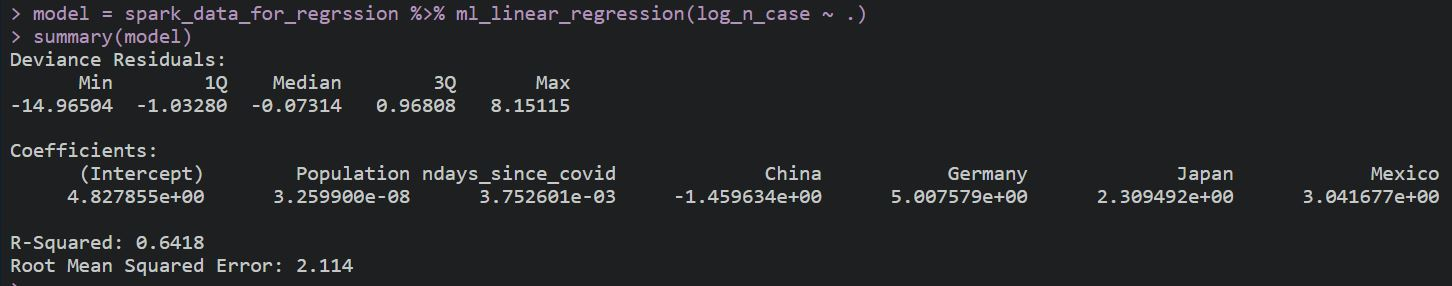
\includegraphics{./ml_regression_summary.JPG}
\caption{Summary of regression analysis.}
\end{figure}

We can see that log number of cases increase with both population and
number of days since COVID begins, which makes sence as there is a
higher chance of infection for countries with denser population and
longer time into the pandemic. For countries, we can see that except
China other countries have more cases than the US. The R-squared
statistic of the model is 0.6418 which means that 64.18\% of the
variation in the dependent variable can be attributed to the independent
variables. In other words, this model is a fairly good fit.

\end{document}
